\documentclass[a4paper, 12pt]{article}

\newcommand{\templates}{../../template}
\usepackage[a4paper, margin=2.5cm]{geometry}

\usepackage{enumitem}
\setlist[itemize]{noitemsep}
\setlist[enumerate]{noitemsep}

\let\oldpar\paragraph
\renewcommand{\paragraph}[1]{\oldpar{#1\\}\noindent}
\usepackage{graphicx}
\usepackage{hyperref}
\usepackage{makecell}

\newcommand{\settitolo}[1]{\newcommand{\titolo}{#1\\}}
\newcommand{\setprogetto}[1]{\newcommand{\progetto}{#1\\}}
\newcommand{\setcommittenti}[1]{\newcommand{\committenti}{#1\\}}
\newcommand{\setredattori}[1]{\newcommand{\redattori}{#1\\}}
\newcommand{\setrevisori}[1]{\newcommand{\revisori}{#1\\}}
\newcommand{\setresponsabili}[1]{\newcommand{\responsabili}{#1\\}}
\newcommand{\setversione}[1]{
	\ifdefined\versione\renewcommand{\versione}{#1\\}
	\else\newcommand{\versione}{#1\\}\fi
}
\newcommand{\setdestuso}[1]{\newcommand{\uso}{#1\\}}
\newcommand{\setdescrizione}[1]{\newcommand{\descrizione}{#1\\}}

\newcommand{\makefrontpage}{
	\begin{titlepage}
		\begin{center}

		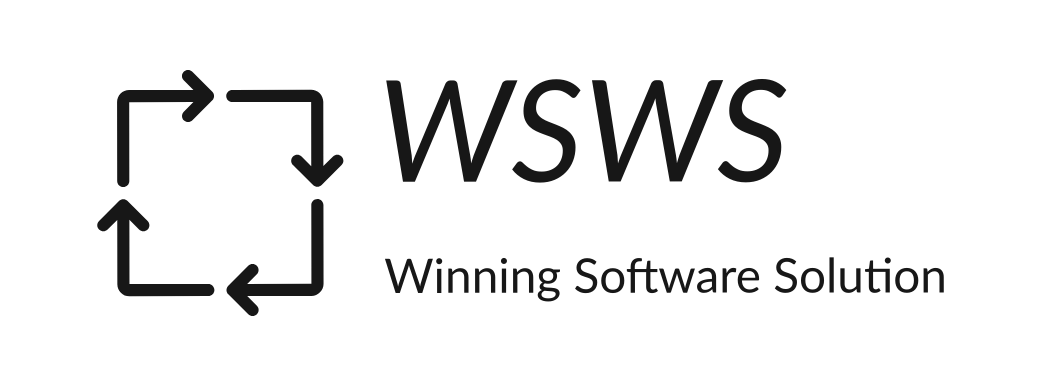
\includegraphics[width=0.4\textwidth]{../../template/WSWS-logos_transparent_crop}\\

		{\Large Winning Software Solution}\\[6pt]
		\href{mailto://winningsoftwaresolution@gmail.com}{winningsoftwaresolution@gmail.com}\\
		
		\ifdefined\progetto
		\vspace{1cm}
		{\Large\progetto}
		{\large\committenti}
		\else\fi
		
		\vspace{1.5cm}
		{\LARGE\titolo}
		
		\vfill
		
		\begin{tabular}{r | l}
		\multicolumn{2}{c}{\textit{Informazioni}}\\
		\hline
		
		\ifdefined\redattori
			\textit{Redattori} &
			\makecell[l]{\redattori}\\
		\else\fi
		\ifdefined\revisori
			\textit{Revisori} &
			\makecell[l]{\revisori}\\
		\else\fi
		\ifdefined\responsabili
			\textit{Respondabili} &
			\makecell[l]{\responsabili}\\
		\else\fi
		
		\ifdefined\versione
			\textit{Versione} & \versione
		\else\fi
		
		\textit{Uso} & \uso
		
		\end{tabular}
		
		\vspace{2cm}
		
		\ifdefined\descrizione
		Descrizione
		\vspace{6pt}
		\hrule
		\descrizione
		\else\fi
		\end{center}
	\end{titlepage}
}
\usepackage{hyperref}
\usepackage{array}
\usepackage{tabularx}

\def\vers#1-#2-#3-#4-#5\\{#1&#2&#3&#4&#5\\\hline}

\newcommand{\addversione}[5]{
	\ifdefined\versioni
		\let\old\versioni
		\renewcommand{\versioni}{#1&#2&#3&#4&#5\\\hline\old}
	\else
		\newcommand{\versioni}{#1&#2&#3&#4&#5\\\hline}
	\fi
}

\newcommand{\setversioni}[1]{\newcommand{\versioni}{#1}}

\newcommand{\makeversioni}{
	\begin{center}
		\begin{tabularx}{\textwidth}{|c|c|c|c|X|}
		\hline
		\textbf{Versione} & \textbf{Data} & \textbf{Persona} & \textbf{Attivtà} & \textbf{Descrizione} \\
		\hline
		\versioni
		\end{tabularx}
	\end{center}
	\clearpage
}

%package
\usepackage[table,xcdraw]{xcolor}

\settitolo{Analisi delle tecnologie}
\setredattori{Federico Marchi \\ Matteo Galvagni}
\setdestuso{interno}
\setdescrizione{
Analisi delle tecnologie.
}

\begin{document}

\makefrontpage

\section{Analisi delle Blockchain}
\subsection*{Premesse}

\renewcommand\arraystretch{1.6}

%Tabella scalabilità
\begin{center}
\begin{tabular}{lc
>{\columncolor[HTML]{ADE694}}c
>{\columncolor[HTML]{ADE694}}c
>{\columncolor[HTML]{ADE694}}c c
>{\columncolor[HTML]{ADE694}}c }
& \multicolumn{1}{l}{}                            & \multicolumn{5}{c}{\cellcolor[HTML]{D1D1D1}\textbf{Scalability}}    \\
\cellcolor[HTML]{D1D1D1}\textbf{BlockChain} & \cellcolor[HTML]{D1D1D1}\textbf{Type}           & \cellcolor[HTML]{EFEFEF}\textbf{Thx fee} & \cellcolor[HTML]{FFFFFF}\textbf{Thx time} & \cellcolor[HTML]{EFEFEF}\textbf{Block Time} & \cellcolor[HTML]{FFFFFF}\textbf{Block Size}      & \cellcolor[HTML]{EFEFEF}\textbf{TPS}       \\
\cellcolor[HTML]{EFEFEF}Ethereum            & \cellcolor[HTML]{EFEFEF}L1                      & \cellcolor[HTML]{FF8F8C}13\$    & \cellcolor[HTML]{FF8F8C}3m       & \cellcolor[HTML]{FFDD99}12s - 15s  & \cellcolor[HTML]{ADE694}$\sim$66 KBytes & \cellcolor[HTML]{FF8F8C}$\sim$15  \\
Polygon                                     & L2 (ETH)                                 & \textless{}0.001\$              & 6s                               & 1-2s                               & \cellcolor[HTML]{ADE694}$\sim$82 KBytes & $\sim$7.2k                        \\
\cellcolor[HTML]{EFEFEF}xDai                & \cellcolor[HTML]{EFEFEF}L2 (ETH)         & \textless{}0.001\$              & 5s                               & 5s                                 & \cellcolor[HTML]{ADE694}$\sim$66 KBytes & \cellcolor[HTML]{FFDD99}$\sim$90  \\
Solana                                      & L1                                              & 0.0025\$                        & 2s                               & 2-6s                               & \cellcolor[HTML]{ADE694}$\sim$64 KBytes & $\sim$50k                         \\
\cellcolor[HTML]{EFEFEF}Algorand            & \cellcolor[HTML]{EFEFEF}L1                      & \textless{}0.01\$               & 5s                               & 4.5s                               & \cellcolor[HTML]{FF8F8C}$\sim$1 MByte   & $\sim$1k                          \\
Avalanche                                   & L1                                              & \cellcolor[HTML]{FFDD99}0.3\$   & \textless{}1s                    & \cellcolor[HTML]{D9D9D9}-          & \cellcolor[HTML]{FF8F8C}$\sim$1 MByte   & $\sim$4.5k                        \\
\cellcolor[HTML]{EFEFEF}Fantom              & \cellcolor[HTML]{EFEFEF}L1                      & \textless{}0.01\$               & 1s                               & 1-2s                               & \cellcolor[HTML]{FFDD99}$\sim$4 KBytes  & $\sim$10k                         \\
Cardano                                     & L1                                              & \cellcolor[HTML]{FFDD99}0.5\$   & \cellcolor[HTML]{FFDD99}20s      & 4s                                 & \cellcolor[HTML]{ADE694}$\sim$72 KBytes & \cellcolor[HTML]{FFDD99}$\sim$250 \\
\cellcolor[HTML]{EFEFEF}Harmony             & \multicolumn{1}{c}{\cellcolor[HTML]{EFEFEF}L1} & \textless{}0.001\$            & 1-2s                             & 2-3s                               & \cellcolor[HTML]{FF8F8C}$\sim$2 MBytes  & $\sim$8k
\end{tabular}
\end{center}

%Tabella Sicurezza & decentralizzazione
\begin{center}
\begin{tabular}{lc
>{\columncolor[HTML]{ADE694}}c cc}
& \multicolumn{1}{l}{}                            & \multicolumn{3}{c}{\cellcolor[HTML]{D1D1D1}\textbf{Security \& Decentralization}}                                               \\
\cellcolor[HTML]{D1D1D1}\textbf{BlockChain} & \cellcolor[HTML]{D1D1D1}\textbf{Type}           & \cellcolor[HTML]{FFFFFF}\textbf{\phantom . Consensus  \phantom . } & \cellcolor[HTML]{EFEFEF}\textbf{Miners/Validators} & \cellcolor[HTML]{FFFFFF}\textbf{Top 100 Wallet}         \\
\cellcolor[HTML]{EFEFEF}Ethereum            & \cellcolor[HTML]{EFEFEF}L1                      & \cellcolor[HTML]{FFDD99}POW       & \cellcolor[HTML]{ADE694}1 500 000         & \cellcolor[HTML]{ADE694}$\sim$12.66\% of Supply \\
Polygon                                     & L2 (ETH)                                        & POS                               & \cellcolor[HTML]{FF8F8C}100               & \cellcolor[HTML]{ADE694}$\sim$7.5\% of Supply   \\
\cellcolor[HTML]{EFEFEF}xDai                & \cellcolor[HTML]{EFEFEF}L2 (ETH)                & POS                               & \cellcolor[HTML]{FF8F8C}24                & \cellcolor[HTML]{ADE694}$\sim$14\% of Supply    \\
Solana                                      & L1                                              & POS                               & \cellcolor[HTML]{FFDD99}1 272             & \cellcolor[HTML]{FF8F8C}$\sim$30\% of Supply    \\
\cellcolor[HTML]{EFEFEF}Algorand            & \cellcolor[HTML]{EFEFEF}L1                      & POS                               & \cellcolor[HTML]{FF8F8C}380               & \cellcolor[HTML]{FFDD99}$\sim$26\% of Supply    \\
Avalanche                                   & L1                                              & POS                               & \cellcolor[HTML]{FFDD99}1 180             & \cellcolor[HTML]{ADE694}$\sim$9.3\% of Supply   \\
\cellcolor[HTML]{EFEFEF}Fantom              & \cellcolor[HTML]{EFEFEF}L1                      & POS                               & \cellcolor[HTML]{FF8F8C}60                & \cellcolor[HTML]{FFDD99}$\sim$23\% of Supply    \\
Cardano                                     & L1                                              & POS                               & \cellcolor[HTML]{FFDD99}2 965             & \cellcolor[HTML]{ADE694}$\sim$9.94\% of Supply  \\
\cellcolor[HTML]{EFEFEF}Harmony             & \multicolumn{1}{c}{\cellcolor[HTML]{EFEFEF}L1} & POS                               & \cellcolor[HTML]{FF8F8C}280               & \cellcolor[HTML]{FF8F8C}$\sim$40\% of Supply
\end{tabular}
\end{center}


\subsection*{Ethereum}
\subsection*{Polygon}
\subsection*{xDai}
\subsection*{Solana}
\subsection*{Algorand}
\subsection*{Avalanche}
\subsection*{Fantom}
\subsubsection*{Scalabilità}
Si tratta di una blockchain ad alta scalabilità, infatti esegue quasi istantaneamente le transazioni a costi pressoché trascurabili.
\subsubsection*{Sicurezza \& Decentralizzazione}
L' algoritmo di consenso utilizzato si chiama Lachesis, si tratta di un PoS con BTF (Byzantine Fault Tolerance) secondo il quale la blockchain rimane stabile e in funzione fin tanto che i $\frac{2}{3}$ dei validatori non è malevolo.
Da un lato questo algoritmo potrebbe facilitare un'ipotetico attacco alla blockchain, tuttavia essendo complesso e oneroso diventare validatore risulta alla fine complesso e controproducente attaccare la blockchain.
Per poter diventare validatore sono necessari 1 milione di FTM (token nativo di Fantom), circa l’equivalente di 2 milioni di dollari.
Pecca sotto l’aspetto della decentralizzazione poiché sono presenti solo 60 validatori momentaneamente, di cui 10 appartenenti alla Fantom Foundation.
\subsubsection*{Considerazioni finali}
Nonostante sia una delle migliori blockchain sotto il punto di vista della scalabilità, non è stata scelta poiché riteniamo, al fine di garantire una lunga prospettiva di vita al progetto, che sia fondamentale utilizzare una blockchain maggiormente decentralizzata, dunque con un numero di validatori superiore.
\subsection*{Cardano}
\subsection*{Harmony}
\section{Analisi seconda tecnologia}
\end{document}
